\subsection{Métodos de reducción de dimensionalidad}

La reducción de dimensionalidad es un proceso que disminuye el tamaño de variables o que describen a un conjunto de datos. Las ventajas de la reducción de dimensionalidad son las siguientes:

\begin{itemize}
    \item Reduce el espacio de tiempo y almacenamiento requerido.
    \item La eliminación de multicolinealidad mejora el rendimiento del modelo de aprendizaje automático.
    \item Se hace más fácil de visualizar los datos cuando se reduce dos o tres dimensiones.
\end{itemize}

Los métodos que se empleo en este trabajo fueron ISOMAP, K-means, Self-Organizing-Map (SOM), T-SNE y análisis de componentes principales (PCA).

\subsubsection{ISOMAP}

Se aplicó el algoritmo ISOMAP descrito en la sección \ref{sec:isomap_theory} con los datos de índice de marginación para los años 2015 y 2020. En la figura \ref{fig:isompa_2d} se observa los resultados del algoritmo para el caso bidimensional para 8, 10, 12 y 14 vecinos.

\begin{figure}[H]
    \centering
    \begin{subfigure}{8.4cm}
        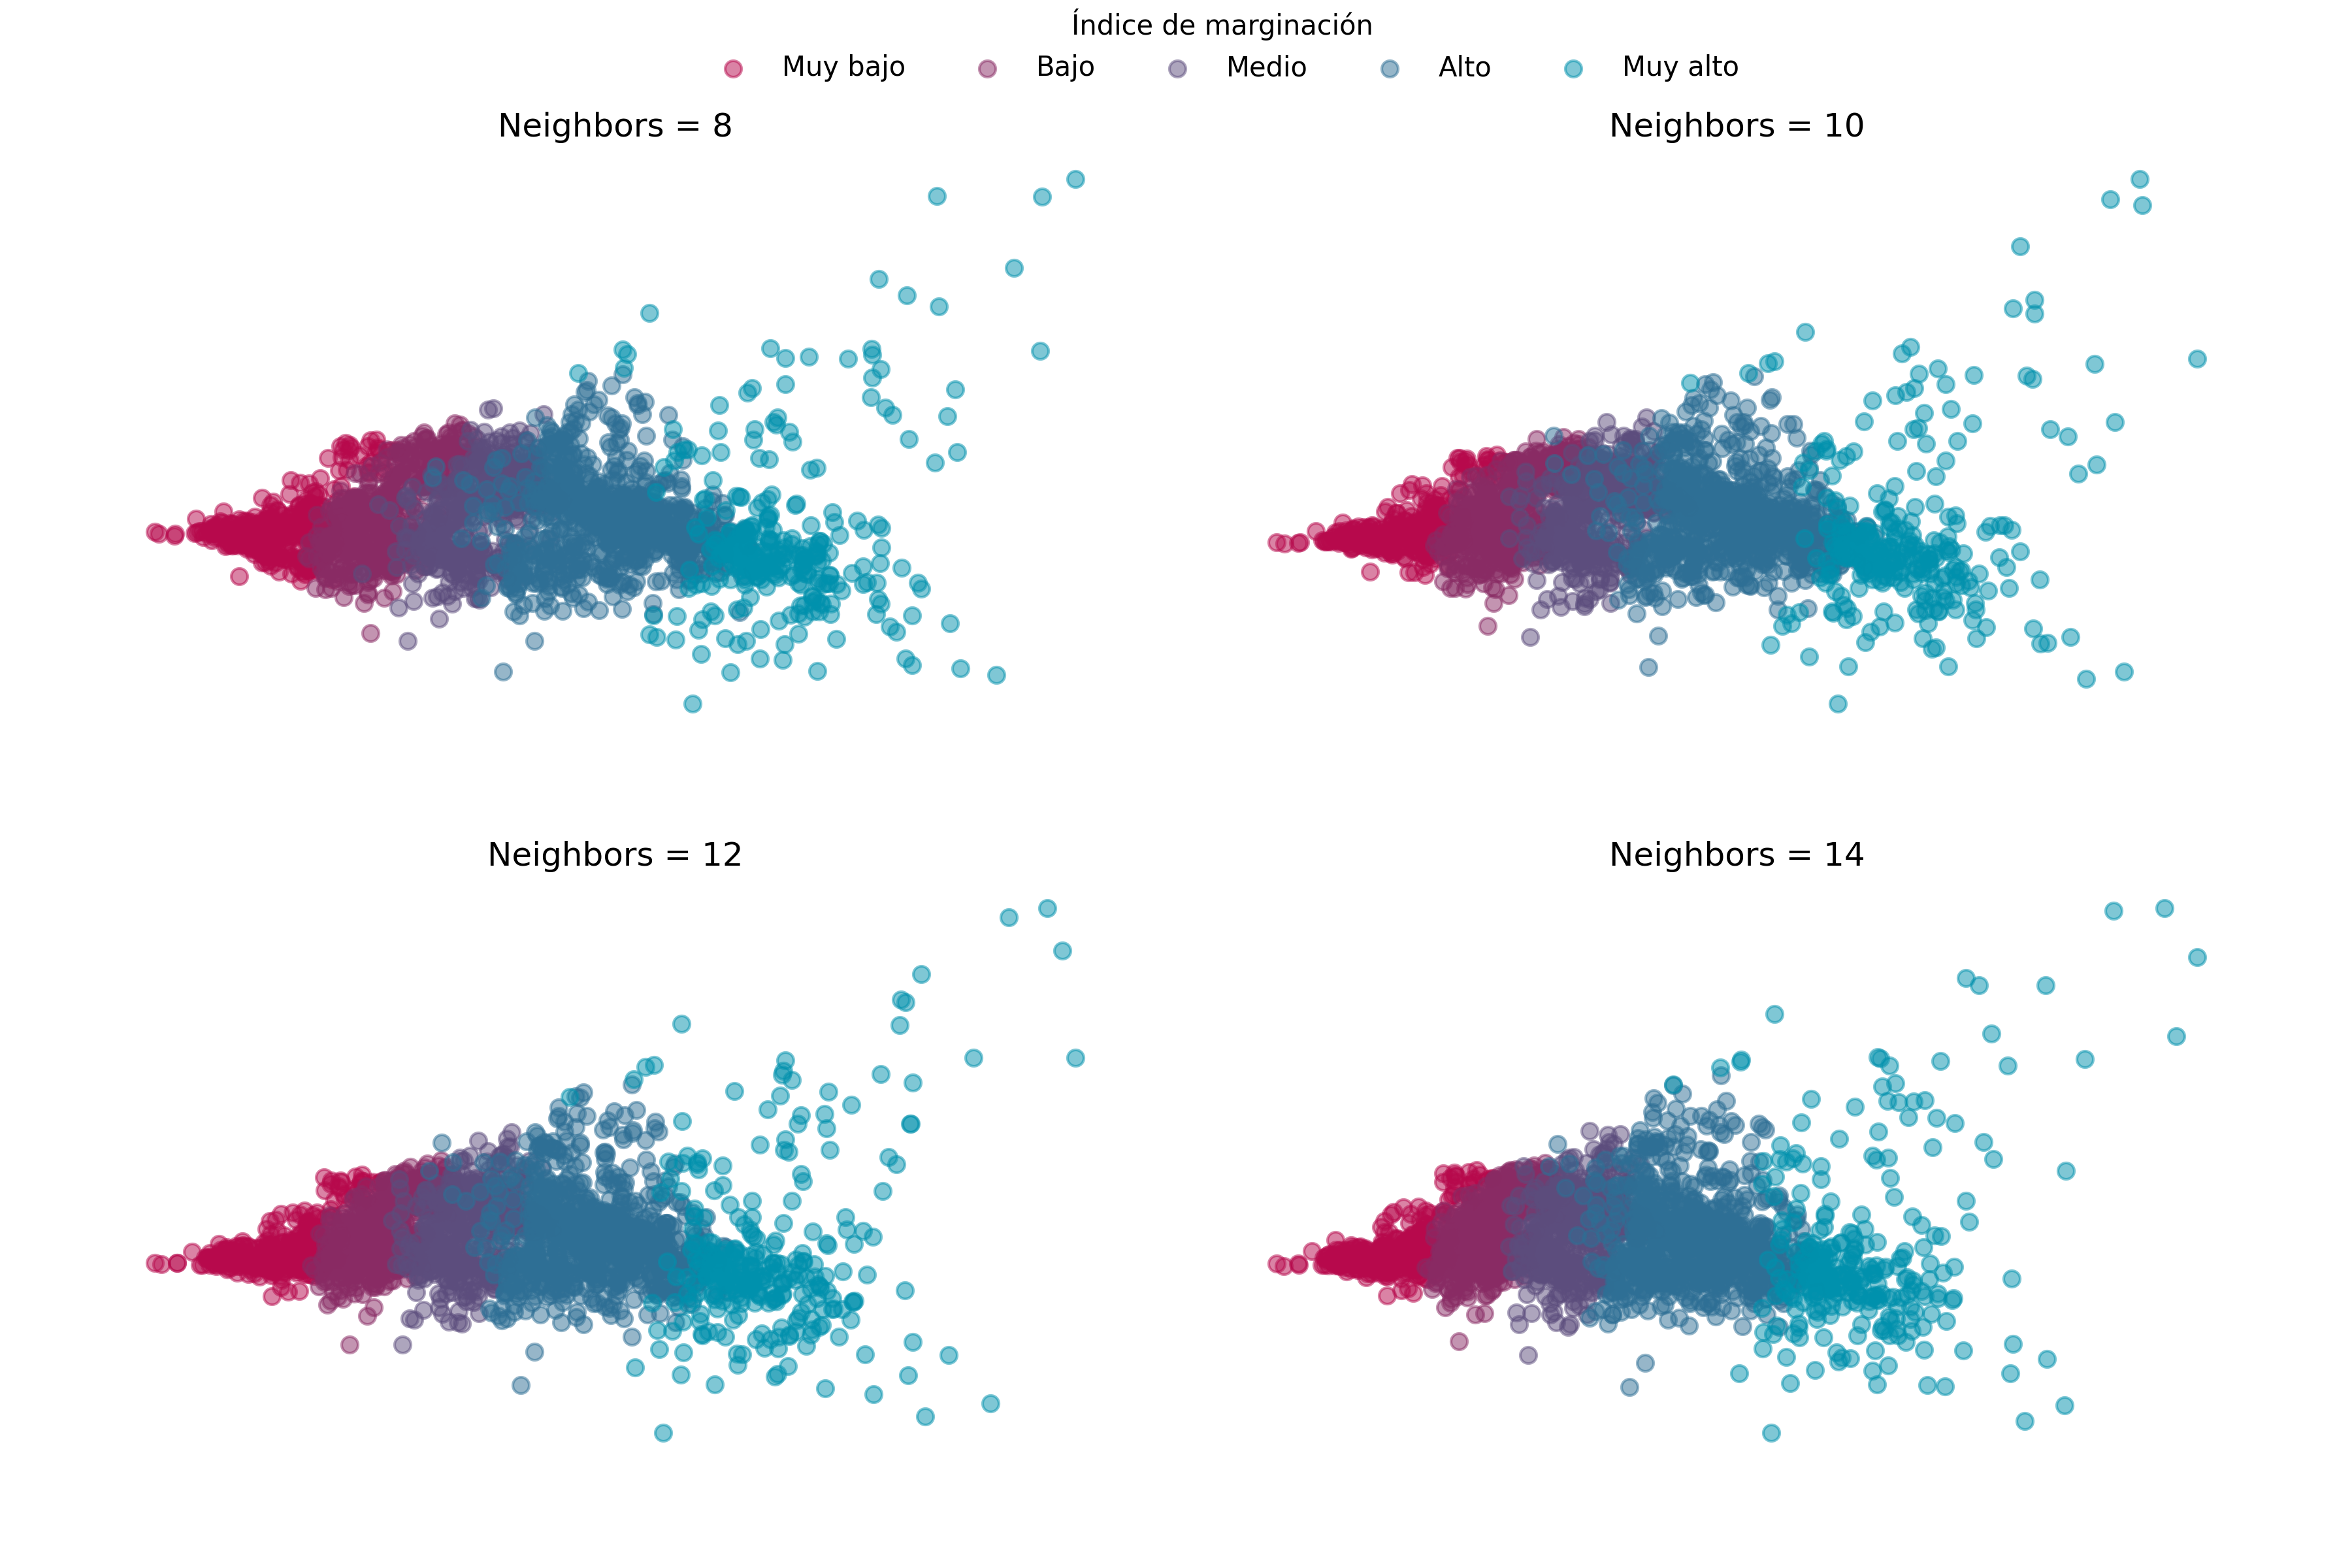
\includegraphics[width=1\linewidth]{Graphics/Data_2015/ISOMAP_2D.png}
        \caption{Datos 2015}
    \end{subfigure}
    \begin{subfigure}{8.4cm}
        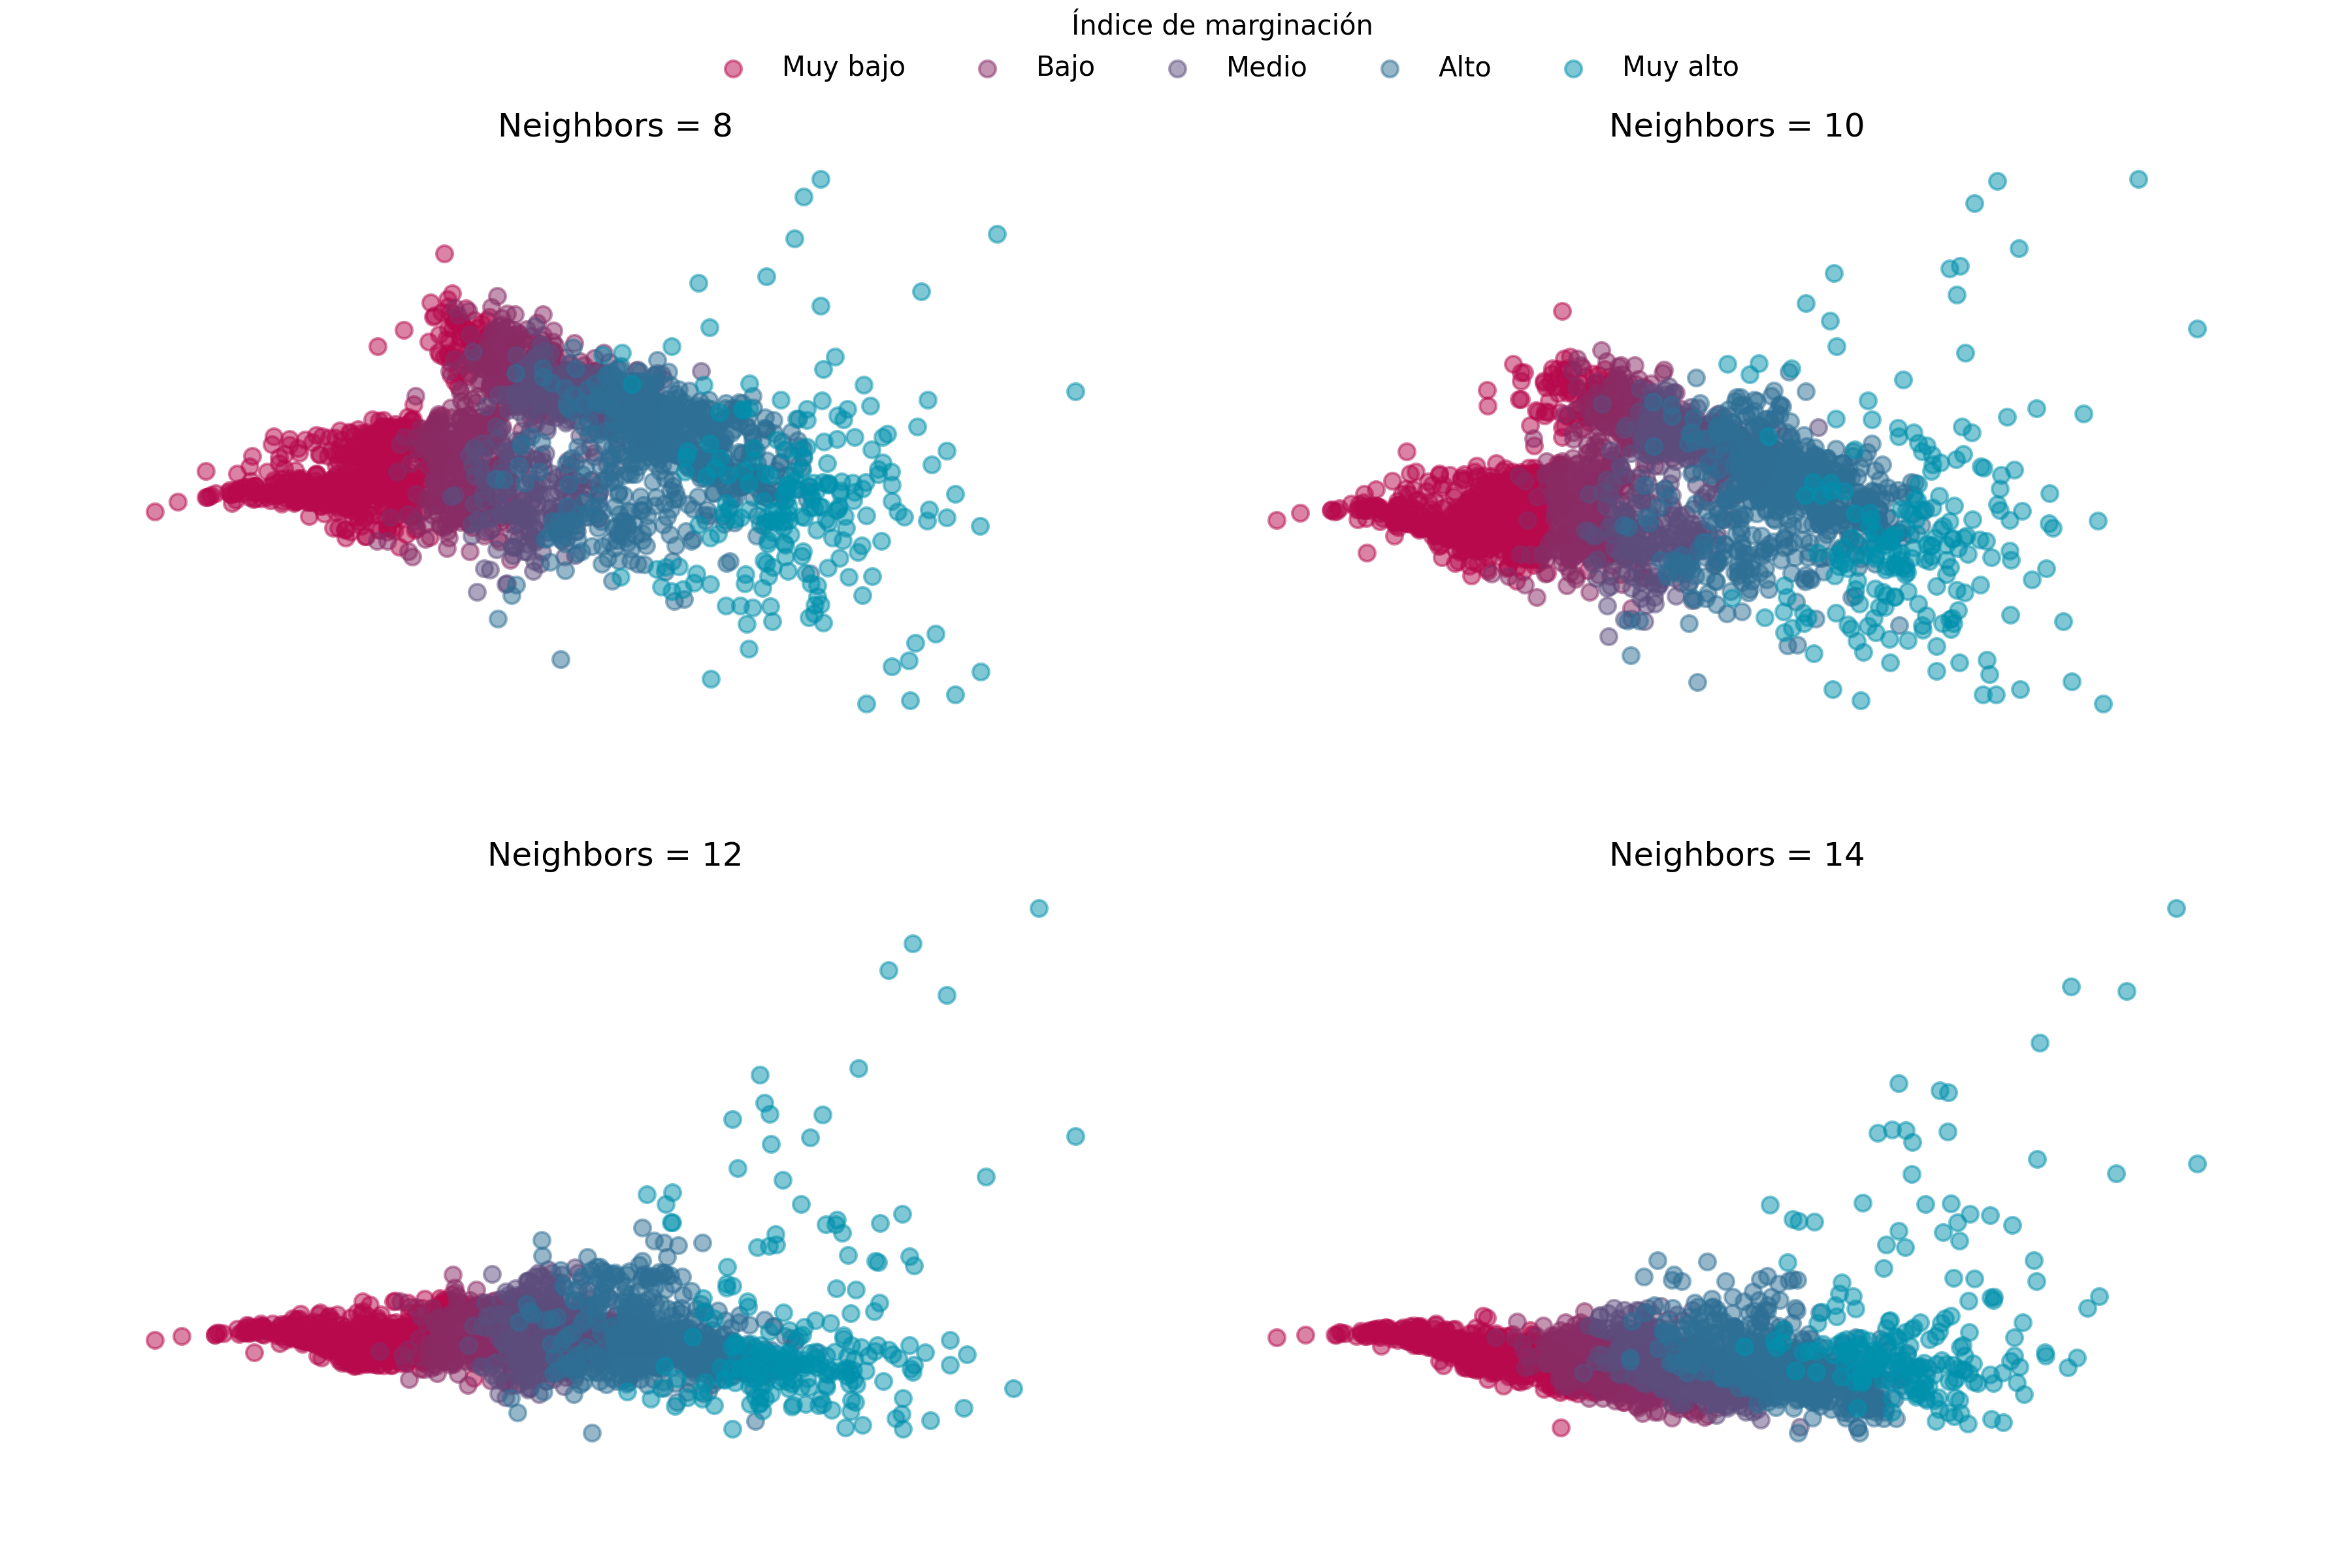
\includegraphics[width=1\linewidth]{Graphics/Data_2020/ISOMAP_2D.png}
        \caption{Datos 2020}
    \end{subfigure}
    \caption{Resultados de aplicar ISOMAP para el caso bidimensional para los datos de índice de marginación de los años 2015 y 2020.}
    \label{fig:isompa_2d}
\end{figure}

En la tabla \ref{table:isomap_results} se pueden descargar las visualizaciones tridimensionales de los resultados del algoritmo ISOMAP en el caso tridimensional para 8, 10, 12 y 14 vecinos para los años 2015 y 2020.

\begin{table}[H]
    \centering
    \begin{tabular}{lrr} \hline
        \multirow{2}{*}{Vecinos} & \multicolumn{2}{c}{Años}                                                                                                                                                                                                                                                \\ \cline{2-3}
                                 & 2015                                                                                                                               & 2020                                                                                                                               \\ \hline
        8                        & \href{https://github.com/giovannilopez9808/Reconocimiento_de_patrones_proyecto/raw/main/Graphics/Data_2015/ISOMAP_3D_8.mp4}{Link}  & \href{https://github.com/giovannilopez9808/Reconocimiento_de_patrones_proyecto/raw/main/Graphics/Data_2020/ISOMAP_3D_8.mp4}{Link}  \\
        10                       & \href{https://github.com/giovannilopez9808/Reconocimiento_de_patrones_proyecto/raw/main/Graphics/Data_2015/ISOMAP_3D_10.mp4}{Link} & \href{https://github.com/giovannilopez9808/Reconocimiento_de_patrones_proyecto/raw/main/Graphics/Data_2020/ISOMAP_3D_10.mp4}{Link} \\
        12                       & \href{https://github.com/giovannilopez9808/Reconocimiento_de_patrones_proyecto/raw/main/Graphics/Data_2015/ISOMAP_3D_12.mp4}{Link} & \href{https://github.com/giovannilopez9808/Reconocimiento_de_patrones_proyecto/raw/main/Graphics/Data_2020/ISOMAP_3D_12.mp4}{Link} \\
        14                       & \href{https://github.com/giovannilopez9808/Reconocimiento_de_patrones_proyecto/raw/main/Graphics/Data_2015/ISOMAP_3D_14.mp4}{Link} & \href{https://github.com/giovannilopez9808/Reconocimiento_de_patrones_proyecto/raw/main/Graphics/Data_2020/ISOMAP_3D_14.mp4}{Link} \\ \hline
    \end{tabular}
    \caption{Link de descarga para las visualizaciones tridimensionales de los resultados de ISOMAP para 8, 10, 12 y 14 vecinos en los años 2015 y 2020.}
    \label{table:isomap_results}
\end{table}

\subsubsection{K-means}

El algoritmo de K-means es un algoritmo de clasificación no supervisada que agrupa objetos en k conjuntos basandose en los valores de las variables dadas. El algoritmo asigna a cada elemento a un conjunto minimizando la suma de las distancias de cada objeto con el centroide del conjunto (ecuación \ref{eq:kmeams_cost_function}).

\begin{equation}
    \underset{\{r_{nk}\}\{\mu_k\}}{min} \sum_{n=1}^N \sum_{k=1}^K r_{nk} ||x_n-\mu_k||^2
    \label{eq:kmeams_cost_function}
\end{equation}

\subsection{Self-Organizing-Map}

\begin{figure}[H]
    \centering
    \begin{subfigure}{8.4cm}
        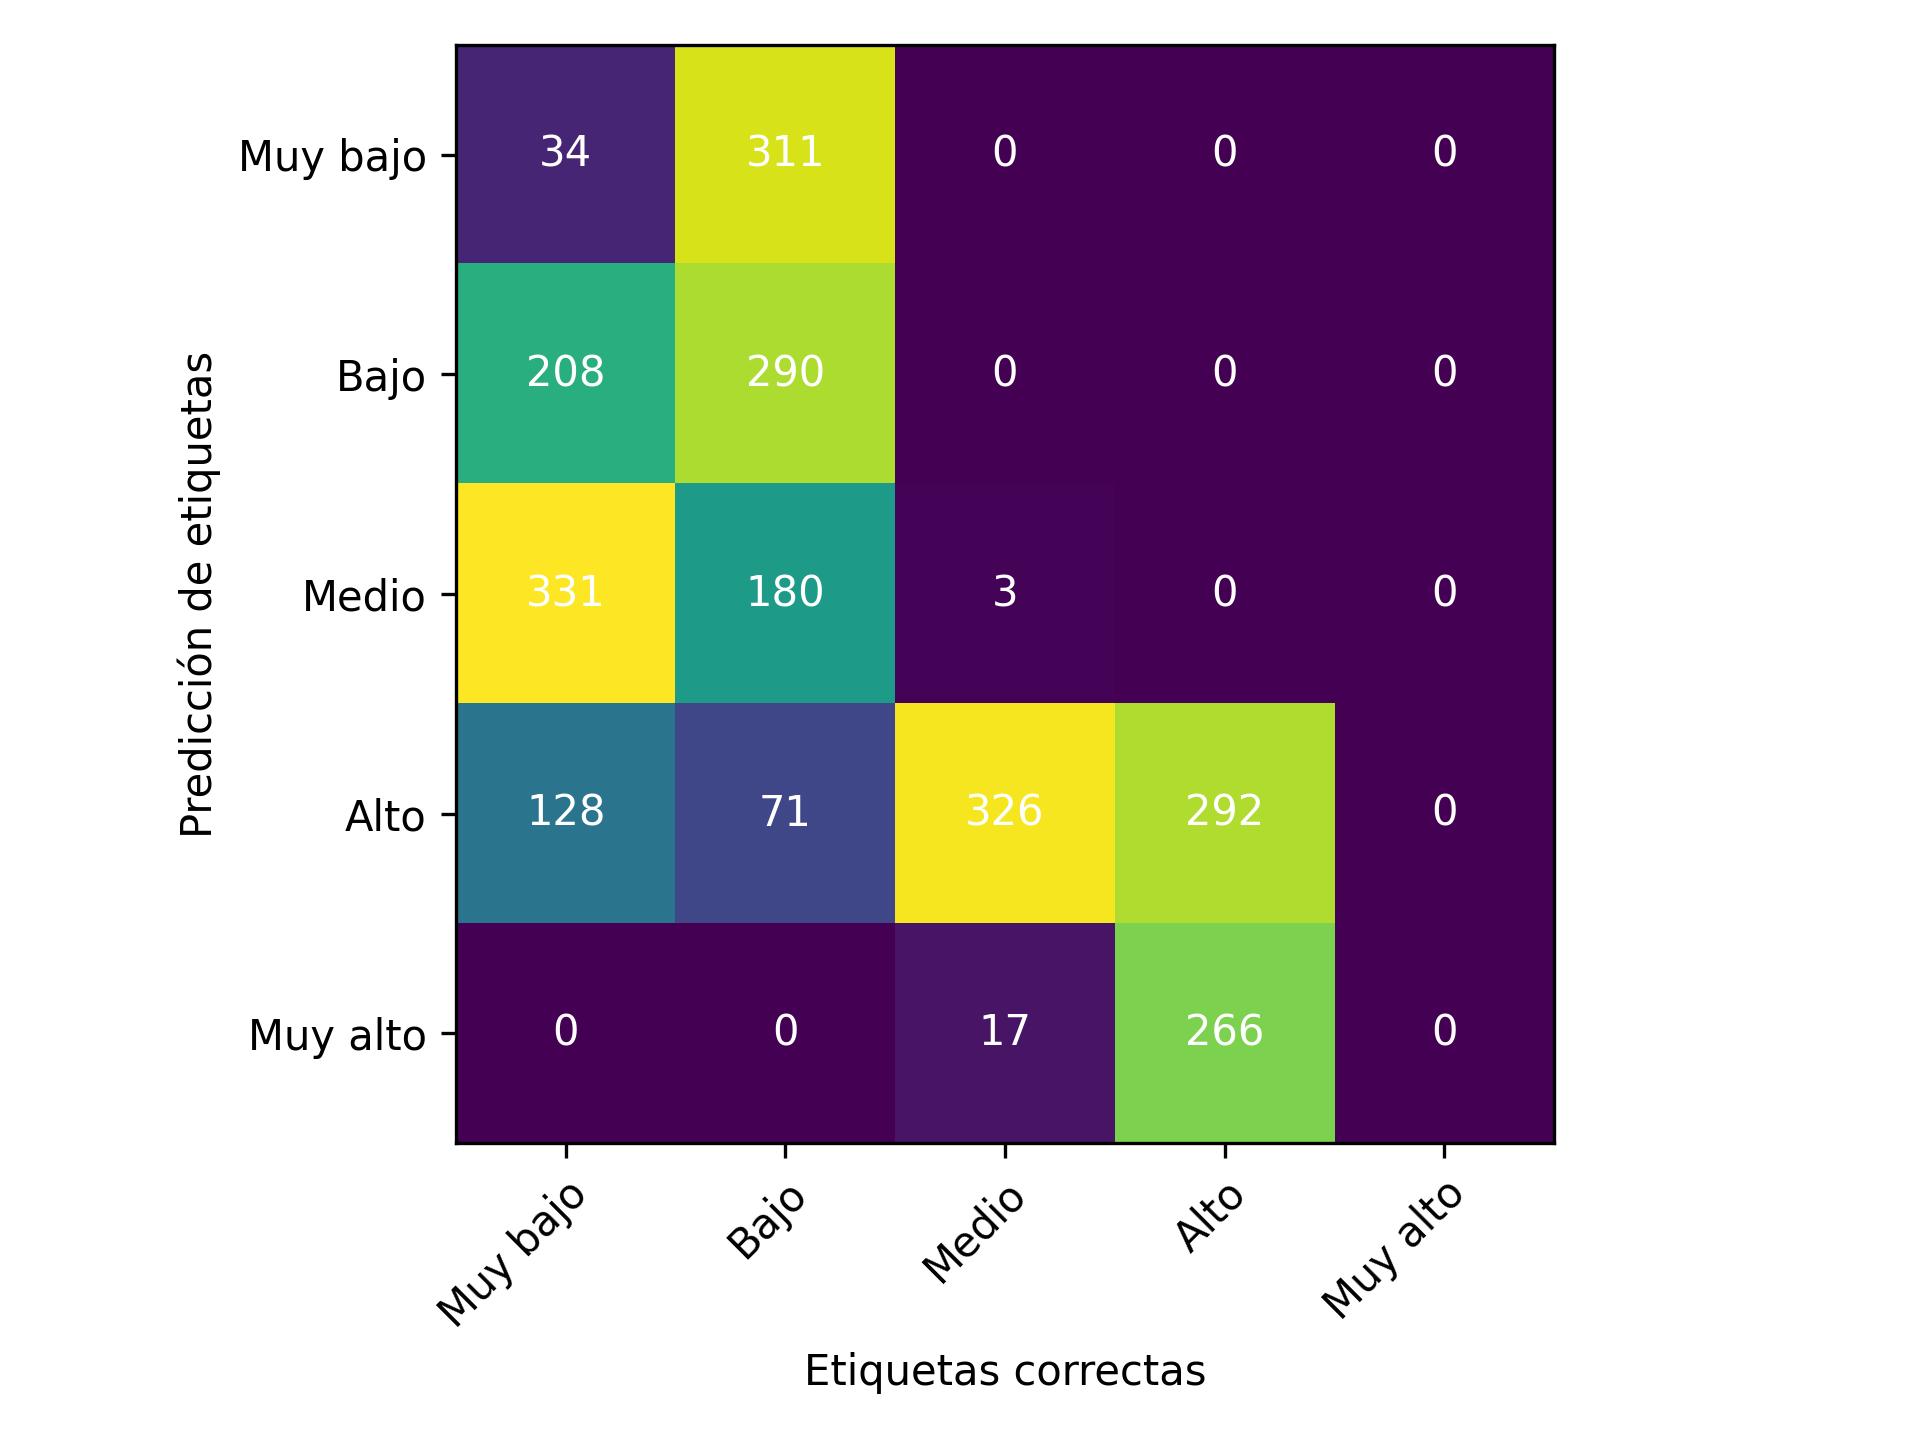
\includegraphics[width=1\linewidth]{Graphics/Data_2015/SOM_confusion_matrix.png}
        \caption{Año 2015}
    \end{subfigure}
    \begin{subfigure}{8.4cm}
        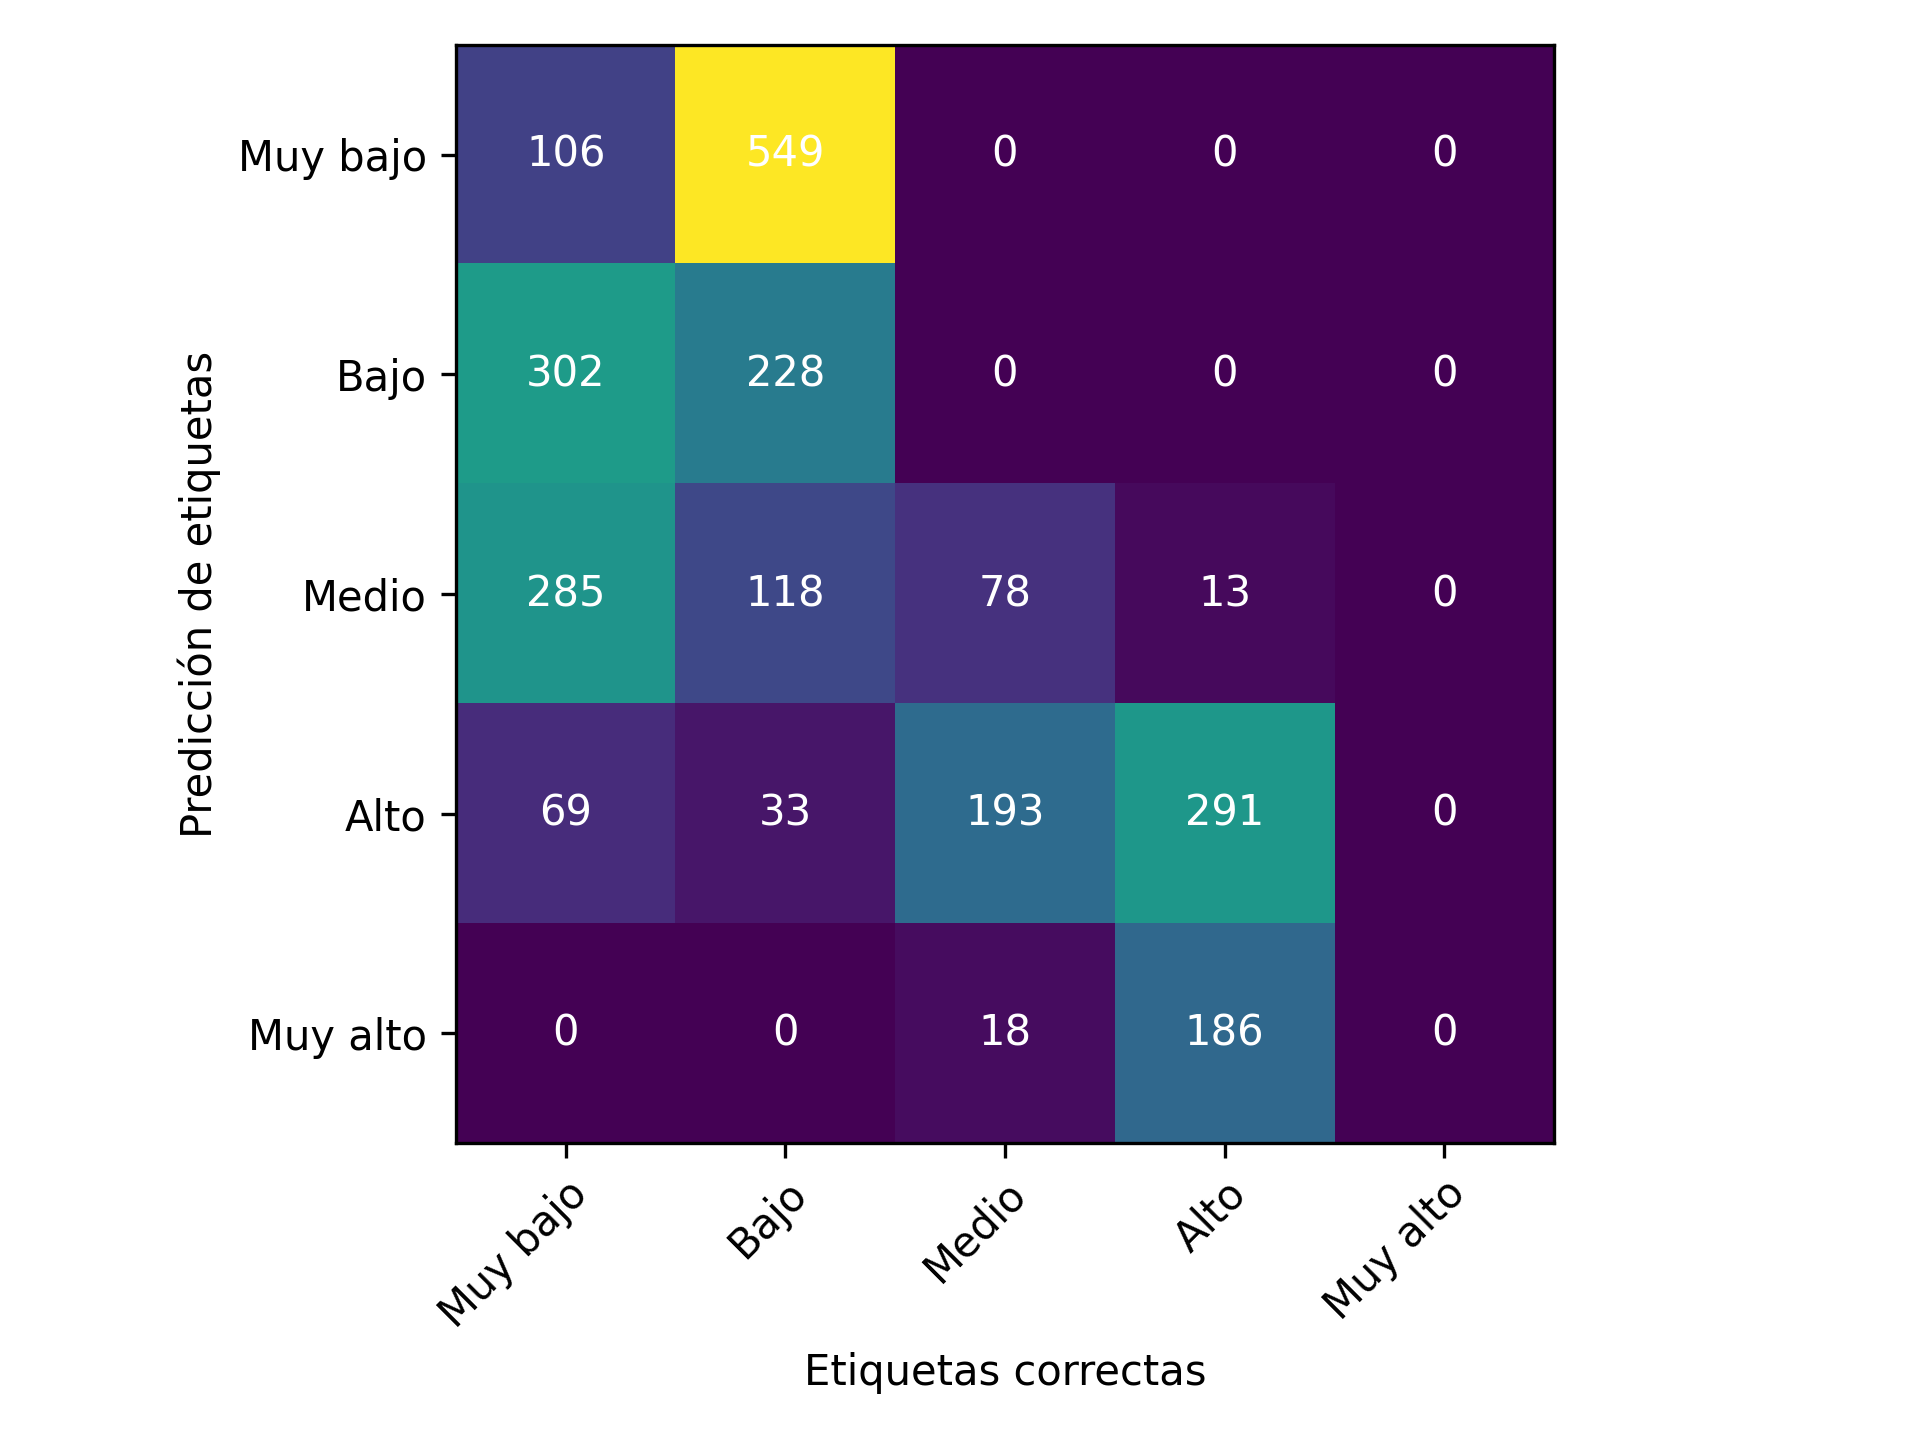
\includegraphics[width=1\linewidth]{Graphics/Data_2020/SOM_confusion_matrix.png}
        \caption{Año 2020}
    \end{subfigure}
    \caption{}
\end{figure}

\pagebreak
\subsubsection{T-SNE}

Se aplicó el algoritmo TSNE descrito en la sección \ref{sec:tsne} con los valores de perplejidad de 100, 200, 300 y 400 con los datos de los años 2015 y 2020. En la figura \ref{fig:tsne_2d} se observan los resultados obtenidos para el caso bidimensional.

\begin{figure}[H]
	\centering
	\begin{subfigure}{8.4cm}
		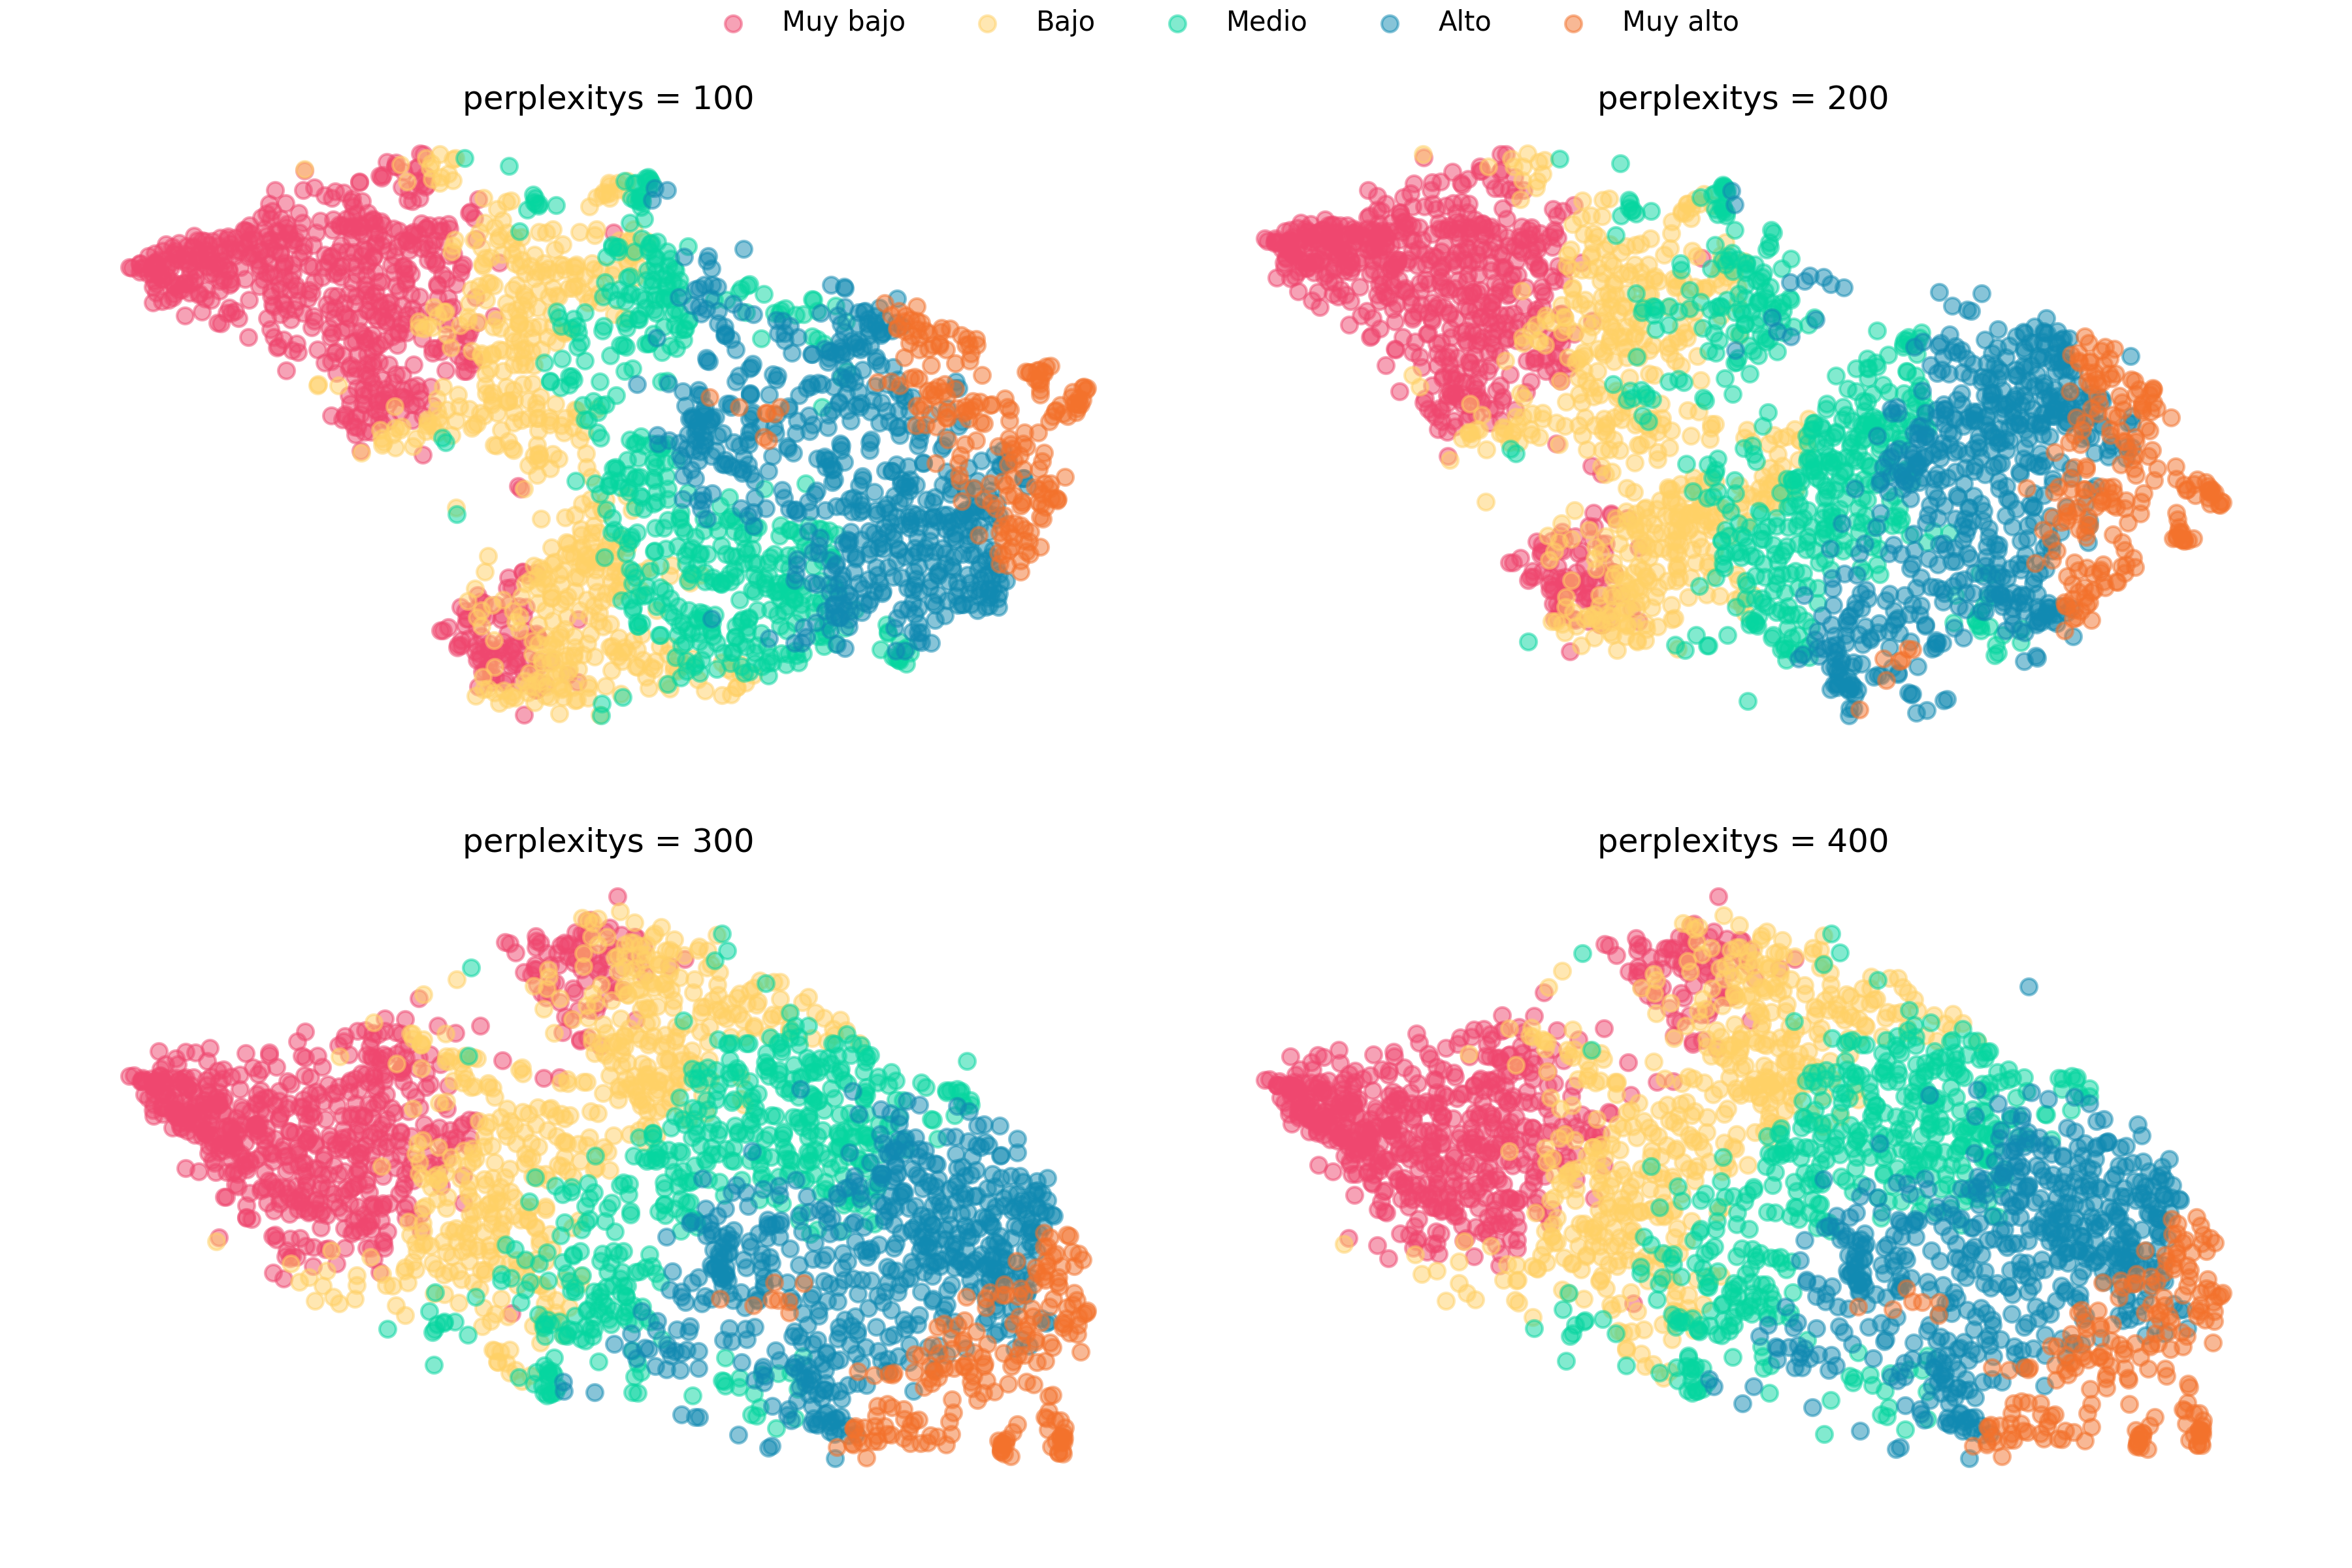
\includegraphics[width=1\linewidth]{Graphics/Data_2015/TSNE_2D.png}
		\caption{Datos 2015}
	\end{subfigure}
	\begin{subfigure}{8.4cm}
		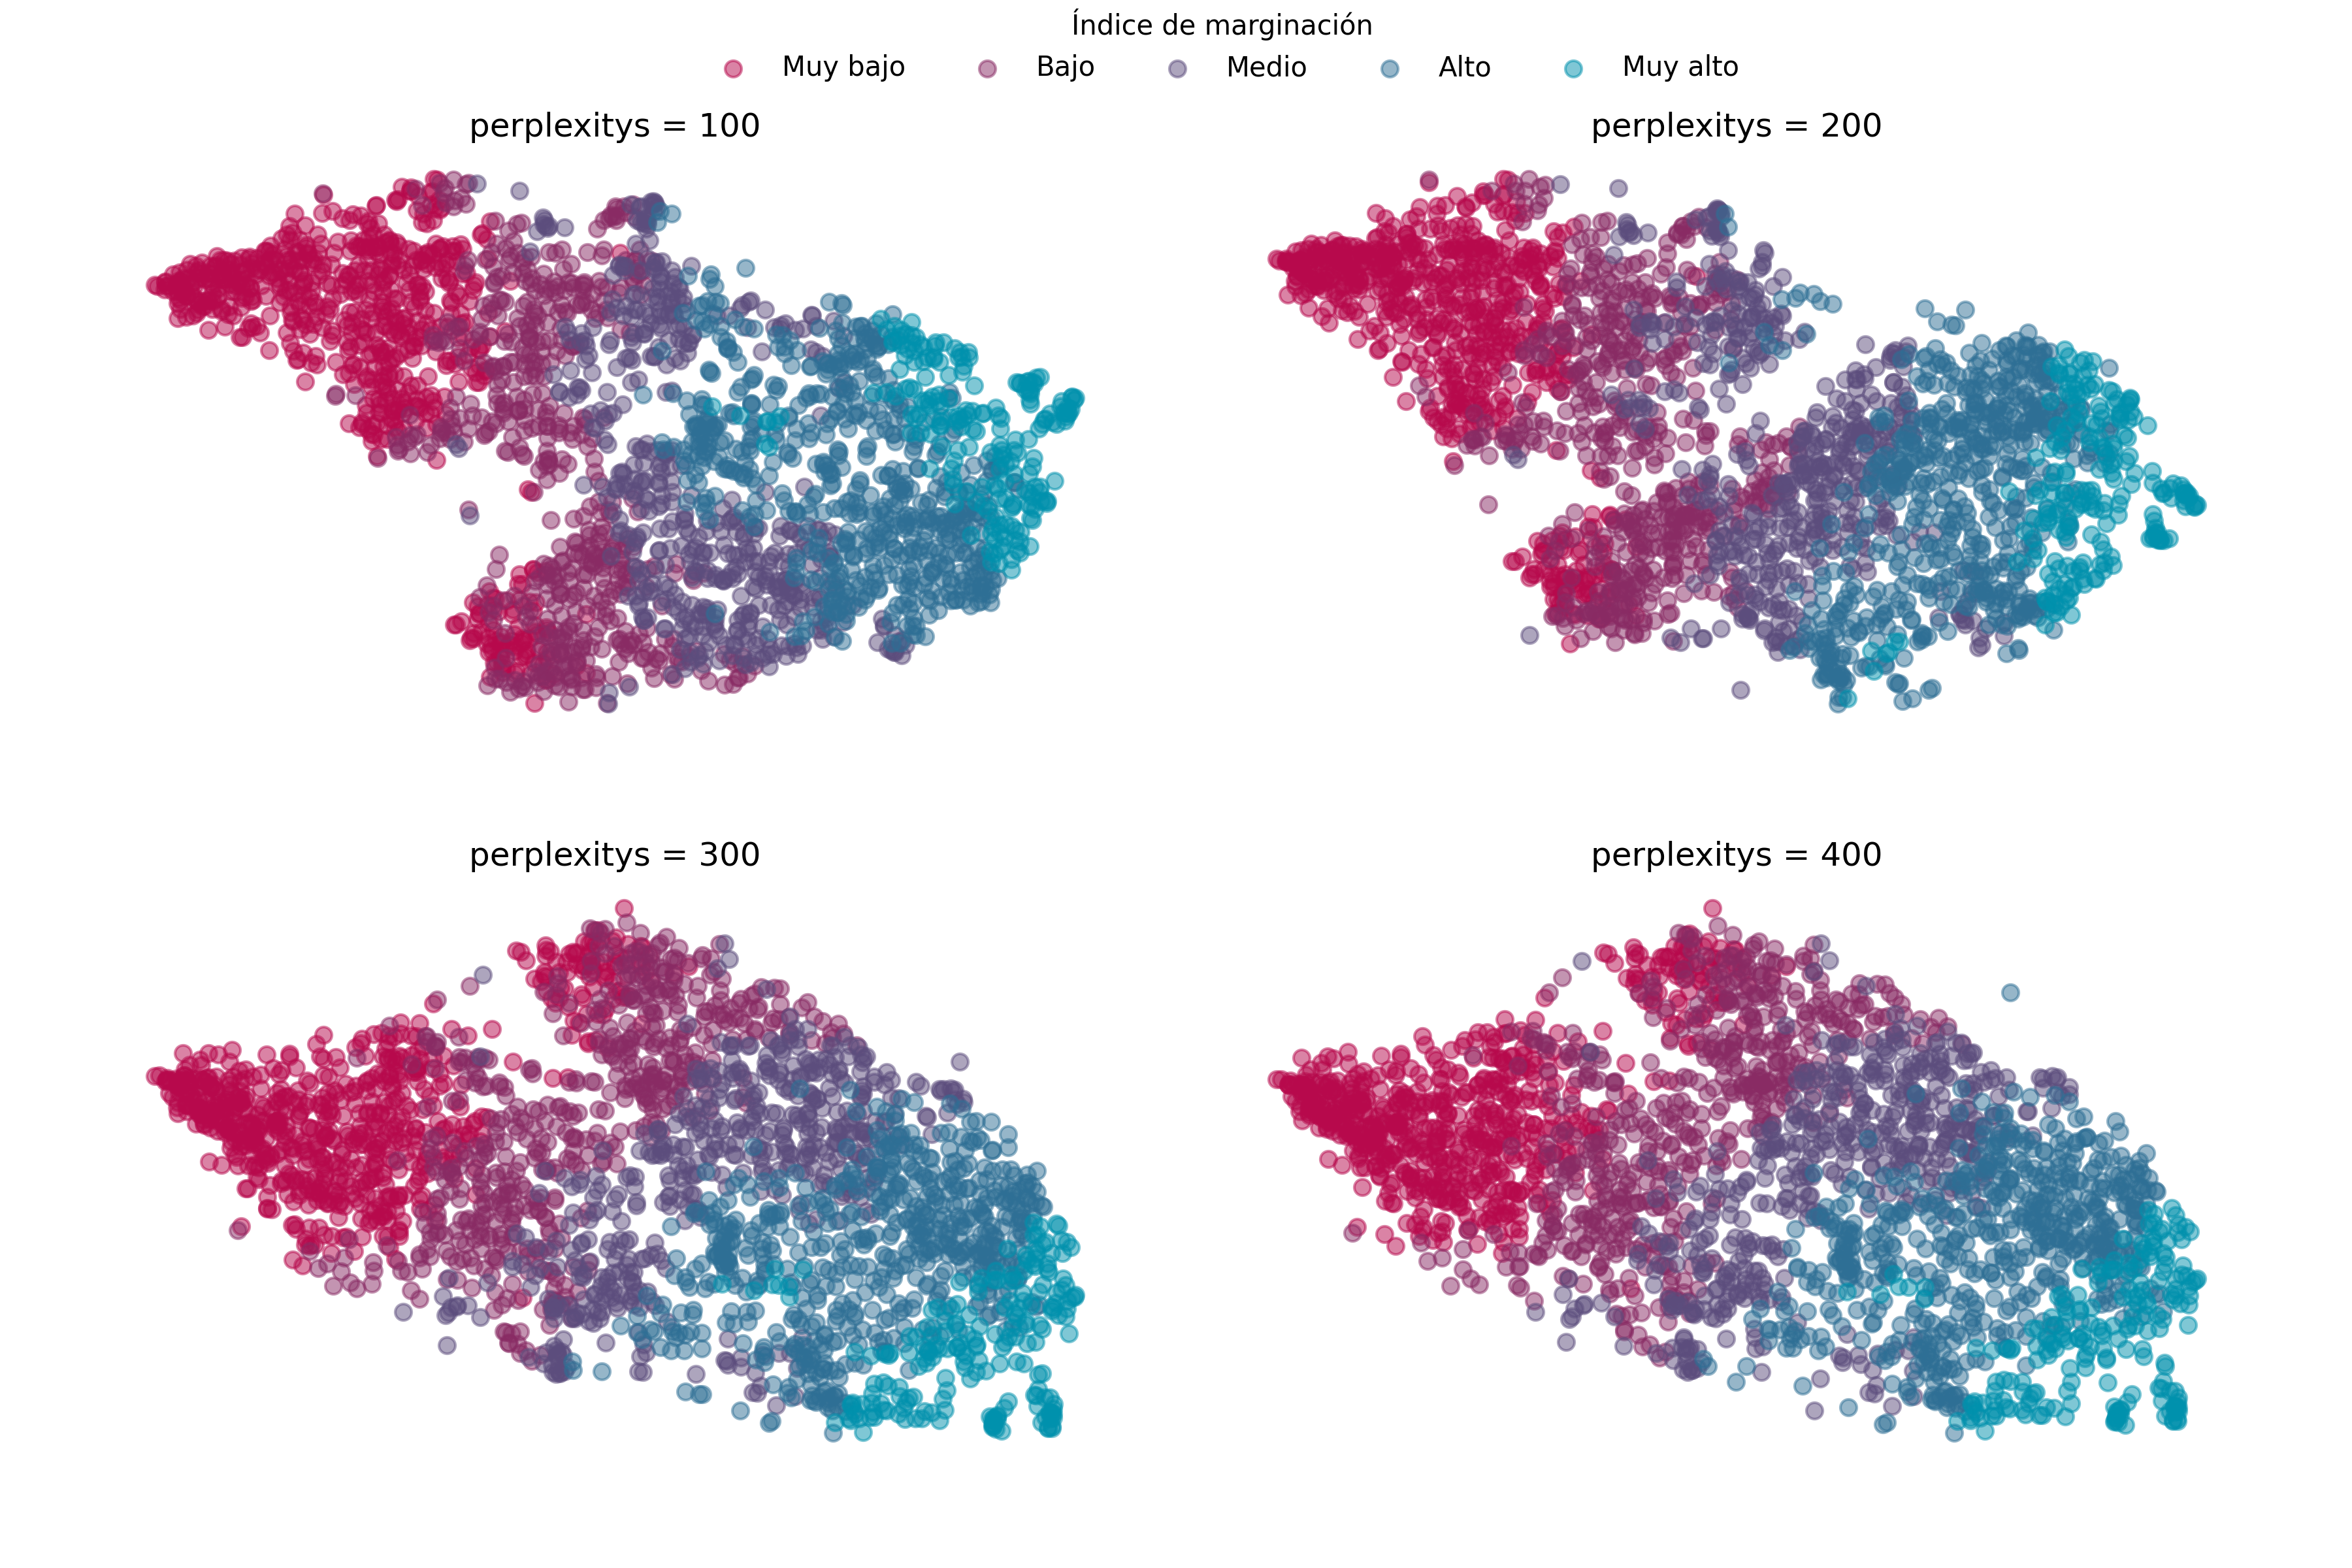
\includegraphics[width=1\linewidth]{Graphics/Data_2020/TSNE_2D.png}
		\caption{Datos 2020}
	\end{subfigure}
	\caption{Resultados de aplicar T-SNE para el caso bidimensional para los datos de índice de marginación de los años 2015 y 2020.}
	\label{fig:tsne_2d}
\end{figure}

En la tabla \ref{table:tsne_results} se pueden descargar las visualizaciones tridimensionales de los resultados del algoritmo ISOMAP en el caso tridimensional.

\begin{table}[H]
	\centering
	\begin{tabular}{lrr} \hline
		\multirow{2}{*}{Perplejidad} & \multicolumn{2}{c}{Años}                                                                                                                                                                                                                                              \\ \cline{2-3}
		                             & 2015                                                                                                                              & 2020                                                                                                                              \\ \hline
		100                          & \href{https://github.com/giovannilopez9808/Reconocimiento_de_patrones_proyecto/raw/main/Graphics/Data_2015/TSNE_3D_100.mp4}{Link} & \href{https://github.com/giovannilopez9808/Reconocimiento_de_patrones_proyecto/raw/main/Graphics/Data_2020/TSNE_3D_100.mp4}{Link} \\
		200                          & \href{https://github.com/giovannilopez9808/Reconocimiento_de_patrones_proyecto/raw/main/Graphics/Data_2015/TSNE_3D_200.mp4}{Link} & \href{https://github.com/giovannilopez9808/Reconocimiento_de_patrones_proyecto/raw/main/Graphics/Data_2020/TSNE_3D_200.mp4}{Link} \\
		300                          & \href{https://github.com/giovannilopez9808/Reconocimiento_de_patrones_proyecto/raw/main/Graphics/Data_2015/TSNE_3D_300.mp4}{Link} & \href{https://github.com/giovannilopez9808/Reconocimiento_de_patrones_proyecto/raw/main/Graphics/Data_2020/TSNE_3D_300.mp4}{Link} \\
		400                          & \href{https://github.com/giovannilopez9808/Reconocimiento_de_patrones_proyecto/raw/main/Graphics/Data_2015/TSNE_3D_400.mp4}{Link} & \href{https://github.com/giovannilopez9808/Reconocimiento_de_patrones_proyecto/raw/main/Graphics/Data_2020/TSNE_3D_400.mp4}{Link} \\ \hline
	\end{tabular}
	\caption{Link de descarga para las visualizaciones tridimensionales de los resultados de T-SNE para 100, 200, 300 y 400 DE perplejidad en los años 2015 y 2020.}
	\label{table:tsne_results}
\end{table}


\subsubsection{Análisis de componentes principales \label{sec:pca}}

El análisis de componentes principales (PCA) es un método estadístico que permite simplificar la complejidad de espacios muestrales con muchas dimensiones a la vez que conserva su información. La idea del algoritmo es asociar a cada elemento de la base de datos con un vector de menor dimensión tal que se minimiza la ecuación \ref{eq:pca_idea}.

\begin{equation}
    \sum_i \sum_j (d(x_i,x_j)^2-d(x^*_i-x_j^*)^2)^2
    \label{eq:pca_idea}
\end{equation}

El problema de minimizar la ecuación \ref*{eq:pca_idea} se puede transformar a la ecuación \ref{eq:pca_problem}.

\begin{equation}
    min\;\; ||-\frac{1}{2}\mathbb{C}(\mathbb{D}^2-\mathbb{D}^{*2})\mathbb{C}||_F^2
    \label{eq:pca_problem}
\end{equation}

Donde $\mathbb{C}$ es la matriz para centrar. Definiendo a la matriz kernel como $\mathbb{K}=\mathbb{X}\mathbb{X}^t$ y $\mathbb{D}$ como la matriz asociada a las distancias, la ecuación \ref{eq:pca_problem} puede escribirse como en la ecuación \ref{eq:pca_cost_function}.

\begin{equation}
    min\;\; ||\mathbb{K}_c-\mathbb{K}^*|| \qquad \mathbb{K}_c = \mathbb{C}\mathbb{K}\mathbb{C}
    \label{eq:pca_cost_function}
\end{equation}

La solución de la ecuación \ref{eq:pca_cost_function} es $\mathbb{K}=\sum\limits_i^p \lambda_i v_i v_i^t $, donde $v_i$ y $\lambda_i$ son los eigenvectores y eigenvalores de $\mathbb{K}$ respectivamente.

\paragraph{Kernel lineal}

El kernel lineal se encuentra definido en la ecuación \ref{eq:kernel_lineal}.

\begin{equation}
    K(x,x') = x \cdot x'
    \label{eq:kernel_lineal}
\end{equation}

\paragraph{Kernel coseno}

El kernel coseno se encuentra definido en la ecuación \ref{eq:kernel_coseno}.

\begin{equation}
    K(x,x') = \frac{x\cdot x'}{||x|| ||x'||}
    \label{eq:kernel_coseno}
\end{equation}

Donde $r$ es un parámetro y $d$ es el grado del polinomio.

\paragraph{Kernel gaussiano}

El kernel gaussiano se encuentra definido en la ecuación \ref{eq:kernel_gaussiano}.

\begin{equation}
    K(x,x') = exp(- \gamma ||x - x'||^2)
    \label{eq:kernel_gaussiano}
\end{equation}

Donde $\gamma$ es un parámetro que controla el comportamiento del kernel. Cuando es muy pequeño el modelo se aproxima al kernel lineal.

\paragraph{Kernel sigmoide}

El kernel sigmoide se encuentra definido en la ecuación \ref{eq:kernel_sigmoide}.

\begin{equation}
    K(x,x') = tanh(\gamma (x \cdot x') +r)
    \label{eq:kernel_sigmoide}
\end{equation}


\paragraph{Parámetros}

En la tabla \ref{table:pca_parameters} se encuentran los parámetros que se usaron para cada kernel antes especificado.

\begin{table}[H]
    \centering
    \begin{tabular}{cccc} \hline
        Kernel    & Grado & $\gamma$      & $r$ \\ \hline
        Lineal    & -     & -             & -   \\
        Coseno    & -     & -             & -   \\
        Gaussiano & -     & $\frac{1}{n}$ & -   \\
        Sigmoide  & -     & $\frac{1}{n}$ & 1   \\ \hline
    \end{tabular}
    \caption{Parámetros usados para cada kernel. El simbolo $-$ indica que no es necesario el parámetro en el kernel.}
    \label{table:pca_parameters}
\end{table}
